\chapter{Code Structure}\label{structure}

Roughly the code structure is displayed in Fig.\ref{graph}. For more accurate and detailed description, run Doxygen utility and refer the generated documentation.


\begin{figure}[H]
	\begin{center}
		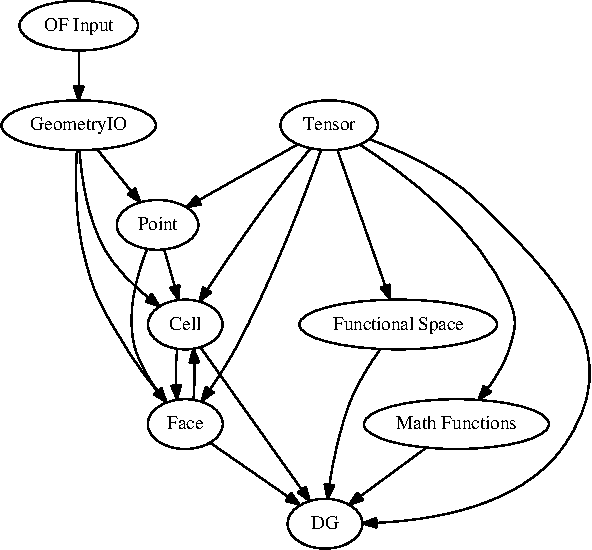
\includegraphics[width=0.8\textwidth]{graph.pdf}
		\caption{\label{graph} Class dependency (crudely)}
	\end{center}
\end{figure}

Each of the the constituent elements are briefly described next. 

\section{Code structure}
\subsection{Tensor}
MEANDG has a central datastructure called as `Tensor', which forms all the important arrays, matrices, multidimensional storage lists etc.
Refer `include/Tensor' for details. Tensor class is made of 4 sub-classes. 
\begin{verbatim}
TensorO1<dType>, TensorO2<dType>, TensorO3<dType>, Matrix<dType>
\end{verbatim}
From these, $O(1), O(2), O(3)$ tensors can be created of arbitrary dimensions. The tensor objects interact with one another and 
have several in-build methods such as $L_1, L_2, L_\infty$ norms etc. All the maths functions accept objects of Tensor library. 

Following example code shows usage of tensor class:
\begin{verbatim}
TensorO1<double> A(5);		// creates a O(1) tensor of size 5 with 
				// data-members of the type double
TensorO1<double> C(5);

for (int i=0; i<5; i++){
	// generate a random number between 0 and 100
	double valueA = getRandom(0.0,100.0);	
	// generate another random number between 0 and 100
	double valueC = getRandom(0.0,100.0);	

	// set value at ith index
	A.setValue(i, valueA);			
	C.setValue(i, valueC);
};
// now A and C have random values 

double dotAnswer = Math::dot(A,C);		// perform math product between two arrays
cout << dotAnswer << endl;			// print the answer


\end{verbatim}

For further details and the available functions, refer the code documentation.

\subsection{Point}
Point is a physical point in $(x,y,z)$ coordiante system. It has a unique id, and description of its location. 

\subsection{Cell}
If the domain is indicated by $\Omega$, then the descritization of the domain ($\Omega_h$) is described as,
\begin{equation}
	\Omega_h = \bigcup\limits_{l = 1}^ n S_i
\end{equation}
where $S_i$ are the finite volume cells. These are non-overlapping pieces of the domain. 
Each cell has the following important attributes (among others):
\begin{itemize}
	\item Vertices (of the type `Point')
	\item Faces (i.e. boundary of the cell)
	\item Degrees of Freedom (i.e. locations where unkowns are evaluated)
	\item Data (such as the conserved variables)
	\item Volume 
	\item Mathematical constructs (Mass matrix, Stiffness matrix etc.)
	\item Mapping onto the standart cell (Jacobian etc.)
\end{itemize}

Thus, each of these parameters (among others) can be accessed using the accessor (get, set) functions of the class `Cell'. 
For further details, refer Cell.h and Cell.cpp.

\subsection{Face}
A face is the boundary of a Cell. The face has following important attributes:
\begin{itemize}
	\item Geometrical information (area, normal, vertices etc.)
	\item Neighbour and Owner cells
	\item Data (numerical flux and variables)
	\item Mapping (Jacobian etc.)
\end{itemize}

\subsection{GeometryIO}
This module reads the input file in the OpenFOAM format and fills the data arrays. Refer:
\begin{verbatim}
GeometryIO::fillDataArrays(args)
\end{verbatim}

\subsection{Functional Space}
This module is responsible for everything related to $L^2, H^1$ functional spaces. It contains nodal, modal basis functions and derivatives.
It also computes various matrices used in DG formulation. 

\subsection{Math functions}
These are various mathematical functions.

\subsection{Gasdynamics, Riemann solvers etc.}
Depending on the system of equations which one wants to solve, include the physics-specific functions and files. For example, for
Euler's equations of Gasdynamics, we have Gasdyanmics.cpp module and corresponding Riemann solvers. 
Apart from these, there are test functions, display functions etc. Refer the code files in `include/' and `src/' folders.

\subsection{DG}
This is the core (central) module of the code. It performs following operations:
\begin{itemize}
	\item Memory management 
	\item Cells, faces creation 
	\item Calling appropriate functions for computation of cell matrices
	\item Time integration
	\item PDE solving
\end{itemize}

Currently it is configured to solve the hyperbolic system of PDEs of the type:
\begin{equation}
	\frac{\partial {Q}}{\partial{t}} + \nabla .  {\bf F}(Q) = 0
\end{equation}

